\chapter{Clasificación de superficies compactas}

\section{Símplices}

\defn{Símplice}{
    Dados $k+1$ puntos $v_0,\dots,v_k\in\R^m$ afínmente independientes, el subconjunto convexo de $\R^m$ más pequeño que los contiene se conoce como un k-símplice y se denota por $\sigma = [v_0, \dots, v_k]$. Los puntos $v_i$ se llaman los vértices del k-símplice. Diremos que la dimensión de $\sigma$ es $k$.
}
\defn{Subsímplices, caras}{
    Si $\sigma=[v_0,\dots,v_k]$ es un k-símplice, cualquier subconjunto no vacío de vértices tambien determina un símplice que llamaremos subsímplice de $\sigma$. Si solo se omite un vértice, el subsímplice correspondiente se denomina una cara.
    \[\text{Las caras de }\sigma\text{ se denotan: } [v_0, \dots, \hat{v}_i, \dots, v_k], \text{ donde } \hat{v}_i \text{ es el vértice omitido.}\]
}

\ex{
    0-símplice (punto), 1-símplice (segmento de línea), 2-símplice (triángulo) y 3-símplice (tetraedro)
    \begin{center}
        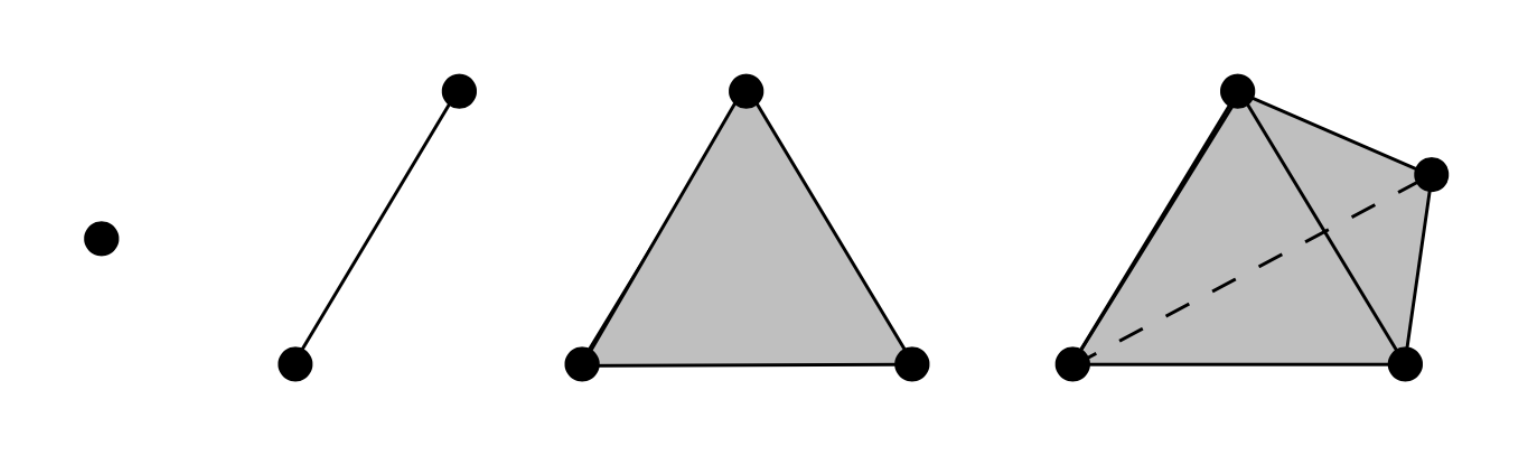
\includegraphics[width=0.7\linewidth]{img/ejemplos-simplices.png}
    \end{center}
}

\defn{Frontera}{
    Si $\sigma=[v_0,\dots,v_k]$ es un k-símplice, la unión de todas sus caras se denomina la frontera de $\sigma$ y se denota por 
    \[\partial\sigma = \displaystyle \bigcup_{0 \le i \le k}[v_0, \dots, \hat{v}_i, \dots, v_k].\]
}
\defn{Interior}{
    Si $\sigma$ es un k-símplice, el complementario de su frontera se denomina el interior de $\sigma$, 
    \[\text{int}(\sigma) = \sigma \setminus \partial\sigma\]
    Inmediatamente, se obtiene $\sigma = \text{int}(\sigma) \cup \partial\sigma$, donde la unión es disjunta.
}

\rmkb{
    La frontera y el interior de un k-símplice \(\sigma\) son conceptos independientes de la topología tomada sobre \(\R^m\). Sin embargo, si \(k = m\), entonces coinciden con la frontera y el interior topológicos de \(\sigma\) en topología usual de \(\R^m\).
}

\section{Complejos simpliciales}

\defn{Complejo simplicial}{
    Un complejo simplicial $K$ es una colección finita de símplices tal que:
    \begin{enumerate}
        \item Cada cara de cada símplice de $K$ también está en $K$.
        \item La intersección de cualesquiera dos símplices de $K$ es vacía o es un subsímplice de ambos.
    \end{enumerate}
    La dimensión de $K$ es la máxima dimensión de sus símplices.
}
\defn{Número de Euler}{
    Sea $K$ un complejo simplicial de dimensión n, si para cada $0 \le k \le n$ denotamos por $i_k$ el número de k-símplices de $K$, entonces el número (o característica) de Euler de $K$ es:
    \[\chi (K) = i_0 - i_1 + \dots + (-1)^n i_n.\]
}
\rmkb{
    Para el caso de un complejo simplicial de dimensión 2, denotando a los vértices $V = i_0$, aristas $E = i_1$ y caras $F=i_2$; la característica de Euler se puede expresar como:
    \[\chi = V - E + F\]
}
\defn{Poliedro asociado}{
    Dado un complejo simplicial $K$, la unión de todos los símplices de $K$ con la topología inducida por la topología usual de $\R^n$ se denomina el poliedro de $K$ y lo denotamos por $|K|$.
}

\section{Triangulaciones}

\defn{Triangulación}{
    Una triangulación de dimensión $n$ de un espacio topológico $X$ es un complejo simplicial $K$ de dimensión $n$ de forma que $|K|$ y $X$ son homeomorfos. En este caso se dice que $X$ es triangulable.
}

Enunciamos el siguiente teorema sin demostración:

\thmr{Teorema de Radó}{rado}{
    Toda superficie topológica admite una triangulación por un complejo simplicial de dimensión 2. Además cada 1-símplice (arista) es subsímplice de exactamente dos 2-símplices (cara).
}

\section{Presentación de superficies}

\defn{Letras y palabras}{
    Sea $A$ un conjunto finito (sus elementos los llamaremos letras). Una palabra $W$ es una sucesión finita de elementos de la forma $a$ ó $a^{-1}$, con $a \in A$, denotada por yuxtaposición.
}

\ex{
    Consideremos el conjunto $A=\{a,b,c\}$ formado por tres letras. Algunos ejemplos de palabras son los siguientes:
    \[W_1=cbab^{-1}ca^{-1},W_2=caab^{-1}bc^{-1},W_3=abb^{-1}a^{-1}.\]
}

\defn{Presentación poligonal}{
    Una presentación poligonal, escrita como $\partes =\langle A|W_1,\dots,W_k\rangle$, está formada por un conjunto finito de letras $A$ y una colección finita de palabras $W_1,\dots,W_k$ que cumplen:
    \begin{enumerate}
        \item Cada letra de $A$ aparece exactamente dos veces en todo el conjunto de palabras.
        \item Cada palabra tiene al menos longitud tres, salvo que haya una sola palabra que podría ser de dos letras.
    \end{enumerate}
}

\clearpage % Para arreglar un espaciado raro

\ex{
    Algunos ejemplos sencillos de presentaciones poligonales son los siguientes:
    \[\partes_1=\langle a\mid  aa^{-1}\rangle, \partes_2=\langle a,b\mid  aba^{-1}b^{-1}\rangle.\]

    \noindent Si consideramos el conjunto de letras y palabras del ejemplo anterior, $\partes=\langle A \mid W_1 \rangle$ es una representación poligonal, pero $\partes'=\langle A \mid W_3 \rangle$ no, ya que la letra $c$ no aparece exactamente dos veces en el conjunto de palabras.
}

\defn{Realización geométrica de $\partes$}{
    Toda presentación poligonal $\partes$ tiene asociado un espacio topológico $|\partes|$ (realización geométrica de $\partes$) construido como sigue: 
    \begin{enumerate}
        \item Para cada palabra se considera un polígono con el mismo número de aristas que la longitud de la palabra. 
        \item Cada arista se etiqueta correlativamente con las letras de la palabra y orientación opuesta si la letra está elevada a -1. 
        \item Finalmente, se identifican las aristas con el mismo nombre y orientación, mediante la topología cociente.
    \end{enumerate}
}

\clmp{}{$|\mathcal{P}|$ es un espacio topológico}{
    Pendiente.
}

\propp{Compacidad y conexión de $|\partes|$}{
    Dada una representación poligonal $\partes$, su realización geométrica, $|\partes|$, es una superficie compacta. Además si solo tiene una palabra, entonces es conexa.
}{
    Vamos a ver que el espacio topológico cociente $\tilde{X}$ es:
    \begin{enumerate}
        \item Compacto
        \item Superficie ($T_2$, $2A\N$, localmente euclídeo)
    \end{enumerate}

    \underline{Compacto:} Sea $X$ el polígono en $\R^2$, sea $\sim$ la relación de equivalencia entre las aristas y sea $\tilde{X}$ el cociente. X es compacto y $p : X \to \tilde{X}=\faktor{X}{\sim}$ la proyección al cociente es continua. Por tanto, $\tilde{X}$ es compacto.

    \underline{$T_2$:} Puedo tomar discos en $\R^2$ infinitamente pequeños de forma que separen los puntos en $X$ y las imágenes por $p$ separan los puntos de $\tilde{X}$.

    \underline{$2A\N$:} La proyección es continua, y el polígono es $2A\N$, luego $\tilde{X}$ también lo es.

    \underline{Localmente euclídeo:} La idea es distinguir 3 casos: 
    \begin{enumerate}
        \item En el interior del polígono: te coges un disco y lo tienes. 
        \item En una arista: te coges medio disco y en la arista con la que se identifique te coges otro medio disco. Vas a juntar Los medios discos en $\R^2$ y el entorno que te coges es el disco con el radio el menor de los dos.
        \item En un vértice: te coges los sectores circulares y el entorno que buscas es un disco en $\R^2$ con el menor radio de esos sectores circulares.
    \end{enumerate}
}
